%----------------------- Wydruk dwustronny ---------------
%\documentclass[12pt,twoside,a4paper]{book} % 
%----------------------- Wydruk jednostronny ---------------
\documentclass[12pt,oneside,a4paper]{book} % jednostronnego

\usepackage{polski}
\usepackage[utf8]{inputenc} %opcja dla edytorów kodujących polskie znaki w utf8
%\usepackage[cp1250]{inputenc} %opcja dla edytorów kodujących polskie znaki w windows-1250
\usepackage{lmodern}
\usepackage{indentfirst}
\usepackage[protrusion=false]{microtype}
\DisableLigatures{encoding = *, family = * }
\usepackage{fancyhdr}
\usepackage{pstricks,graphicx}
\usepackage{amssymb}
\usepackage{float}


%---------------Zbiory liczbowe
\newcommand{\R}{\mathbb{R}}
\newcommand{\N}{\mathbb{N}}
\newcommand{\K}{\mathbb{K}}
\newcommand{\C}{\mathcal{C}}
\newcommand{\p}{\mathcal{P}}
%------------kwantyfikatory--------------
\newcommand{\fal}{\mbox{{\Large $\forall\,$}}}
\newcommand{\ext}{\mbox{{\Large $\exists\,$}}}
%------------------definicje środowisk-----------------
\usepackage{theorem}
\theoremstyle{break}
\theorembodyfont{\it}
\newtheorem{twr}{Twierdzenie}[chapter]
\newtheorem{lem}{Lemat}[chapter]
\theorembodyfont{\rm}
\newtheorem{defi}{Definicja}[chapter]
\newtheorem{wni}{Wniosek}[chapter]
\newtheorem{prz}{Przykład}[chapter]
\newenvironment{dowod}{\par\vspace{0.1cm}\par{ \sc Dowód.}}{\hfill $\blacksquare$\par\vspace{0.4cm}\par}
% ----------ustawienia wymiarow strony
\usepackage{geometry}

\newgeometry{tmargin=2.5cm, bmargin=2.5cm, headheight=14.5pt, inner=3cm, outer=2.5cm} 

\linespread{1.1} %-zmiana interlinii




%---------------- Normalne środowiska --------------------
\usepackage{amsmath}

%----------nagłowki i żywa pagina ------------
\pagestyle{fancy} 
%--------------- Wydruk dwustronny
%\cfoot[]{} 
%\lhead[{\scriptsize{\it \thepage}}]{}
%\chead[{\scriptsize\leftmark}]{{\scriptsize \rightmark}}
%\rhead[]{{\scriptsize{\it \thepage}}}
%--------------- Wydruk jednostronny
\fancyhead[C]{} 
\fancyfoot[C]{\thepage}
\fancyhead[L]{\scriptsize\leftmark}
\fancyhead[R]{\scriptsize\rightmark}

\renewcommand{\chaptermark}[1]{%
\markboth{\MakeUppercase{%
\chaptername}\ \thechapter.%
\ #1}{}}

\usepackage[most]{tcolorbox}
\let\includegraphicsold\includegraphics
\newcommand{\includegraphicsborder}[2][]{\tcbox{\includegraphicsold[#1]{#2}}}

\renewcommand{\sectionmark}[1]{\markright{\thesection.\ #1}}

\usepackage[hidelinks]{hyperref}

\usepackage{graphics}
\graphicspath{ {images/} }

\usepackage{listings}

\renewcommand{\lstlistlistingname}{Spis listingów}
\renewcommand{\lstlistingname}{Listing}

\lstset{
  basicstyle=\footnotesize
}

\usepackage{booktabs}

\newcommand\tabularhead[2]{
  \begin{table}[ht]
    \label{#2}
    \caption{#1}
    \begin{tabular}{|p{0.35\linewidth}|p{0.6\linewidth}|}
    \hline
    \textbf{#1}\\
    \hline
}
\newcommand\addrow[2]{#1 &#2\\ \hline}

\newcommand\addmulrow[2]{ \begin{minipage}[t][][t]{2.5cm}#1\end{minipage}
   &\begin{minipage}[t][][t]{8cm}
    \begin{enumerate} #2   \end{enumerate}
    \end{minipage}\\ }

\newenvironment{usecase}{\tabularhead}
{\hline\end{tabular}\end{table}}



%-----------------właściwa część pracy-----------------
\begin{document}
\thispagestyle{empty}
\begin{center}
  \Large
  \bf{UNIWERSYTET ŚLĄSKI}\\
  \bf{\sf{WYDZIAŁ NAUK ŚCISŁYCH I TECHNICZNYCH}}\\[25mm]
  \large

  \bf{Symulacja Monte Carlo}\\[35mm]

  Sprawozdanie\\[25mm]
\end{center}
\begin{flushright}
  \large
  Autorzy\\
  Kacper Małachowski\\
  Igor Szałas\\[25mm]
\end{flushright}
\begin{center}
  Opracowano:\\
  16.04.2024
\end{center}

\chapter*{Zadanie 1}

Należy zmodyfikować kod dla aproksymacji stałej $\pi$, aby sprawdzić jak rozmiar próbki wpływa na błąd aproksymacji. Błąd aproksymacji obliczamy jako wartość bezwględną różnicy pomiędzy aproksymacją $\pi$ i wartością rzeczywistą $\pi$ (3.14159265). Należy przygotować wykres:

\begin{figure}[H]
  \centering
  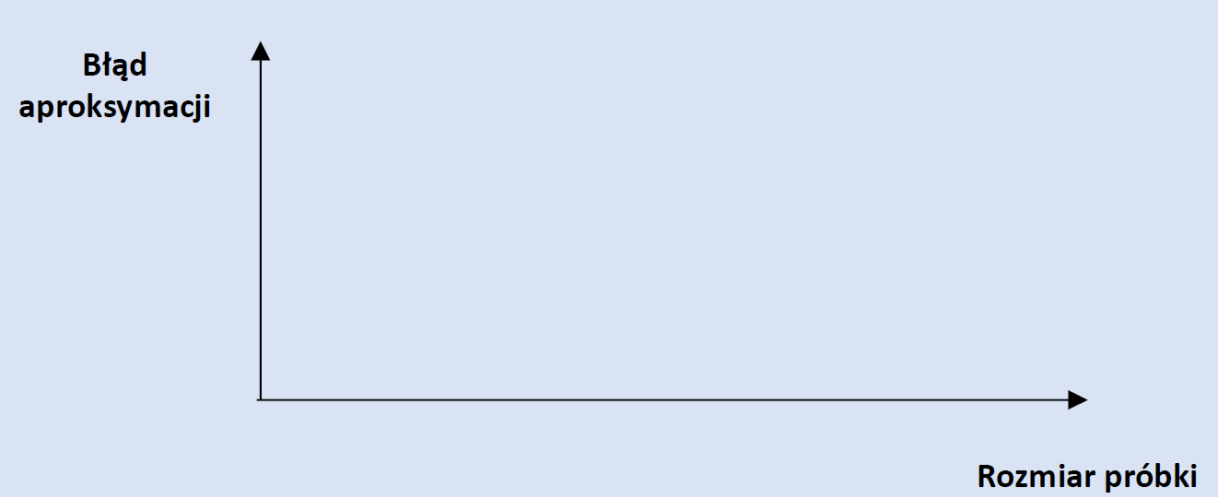
\includegraphics[width=0.75\textwidth]{chart_from_instruction.png}
\end{figure}

\subsection*{Rozwiązanie}

Symulacja została zaprogramowana w języku Python, jako funkcja\\ 'monte\_carlo\_pi\_aproximation' w pliku 'simulation.py'.
Kod tej symulacji przedstawiono poniżej.
\begin{verbatim}
  def monte_carlo_pi_aproximation(runs):
    xs = np.random.uniform(-0.5, 0.5, runs)
    ys = np.random.uniform(-0.5, 0.5, runs)
    inCircle = xs**2 + ys**2 <= 0.5**2

    mcPi = (np.sum(inCircle) / runs) * 4

    return mcPi
\end{verbatim}
Funkcja ta przyjmuje parameter "runs" określający ilość punktów jakie mają być wygenerowane na potrzeby symulacji.

Generuje ona za pomocą metody z pakietu "numpy" losowe punkty w zakresie od $-0.5$ do $0.5$ dla osi "x" oraz osi "y". Ilość punktów wyznacza wartość "runs".

Następnie funkcja wyznacza listę wartości prawda/fałsz, określających obecność danego punktu w okręgu.

Dla stworzenia wynikowego wykresu zaimplementowano ponadto skrypt do uruchamiania symulacji dla różnych wielkości próbek, kod umieszczono poniżej.

\begin{verbatim}
  import numpy as np
  import matplotlib.pyplot as plt
  import simulation as sim

  min_runs = 100000
  increase = 10000
  max_runs = 1000000
  pi_value = 3.14159265

  results = {}

  for runs in range(min_runs, max_runs, increase):
    mc_pi = sim.monte_carlo_pi_aproximation(runs)
    results[runs] = abs(mc_pi - pi_value)

  linear_regression = np.polyfit(
    list(results.keys()), 
    list(results.values()), 
    1
  )

  plt.scatter(results.keys(), results.values())
  plt.plot(
    results.keys(), 
    np.polyval(linear_regression, list(results.keys())), 
    color="red"
  )
  plt.title("Zadanie 1 - Błąd aproksymacji")
  plt.xlabel("Rozmiar próbki")
  plt.ylabel("Błąd aproksymacji")
  plt.savefig("../images/pi_aproximation_based_on_sample_size.png")
\end{verbatim}

W ramach tego skryptu tworzona jest mapa, której kluczami jest ilość próbek w symulacji, a wartościami wyliczony błąd aproksymacji.

Ponadto skrypt ten oblicza i nanosi na wykres linie przedstawiającą regresje liniową wyników.

\newpage
\subsection*{Wyniki}

Ostatecznie uzyskany wykres przedstawiono poniżej.
\begin{figure}[H]
  \centering
  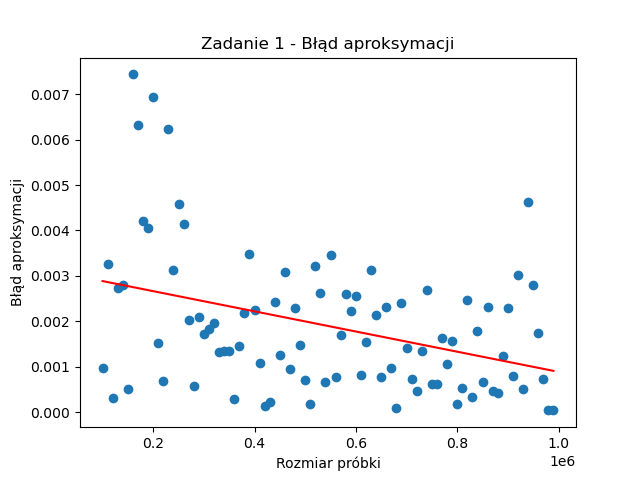
\includegraphics[width=0.75\textwidth]{pi_aproximation_based_on_sample_size.png}
\end{figure}
Dzięki naniesieniu regresji liniowej, widać spadkowy trend błędu aproksymacji wraz ze wzrostem ilości próbek. Ze względu na ilość danych, nie przedstawiono natomiast numerycznych wartości dla każdej próby.

\subsection*{Wnioski}

Wyniki przeprowadzonego zadania pozwalają wysnuć wniosek iż większa liczba próbek znacząco zmniejsza błąd aproksymacji. Szczególnie widoczne jest to na zamieszczonym w ramach zadania wykresie. Naniesione wyniki zarysowują w jaki sposób ilość próbek wpływa na obliczony błąd aproksymacji. W celu lepszego zilustrowania trendu wyników została dodana linia regresu liniowego. 


\chapter*{Zadanie 2}

Zaprogramować symulacje Monte Carlo (np. w języku R), która pozwoli obliczyć pole powierzchni szarego obszaru przedstawionego na poniższym rysunku. Obliczyć błąd uzyskanego wyniku.

\begin{figure}[H]
  \centering
  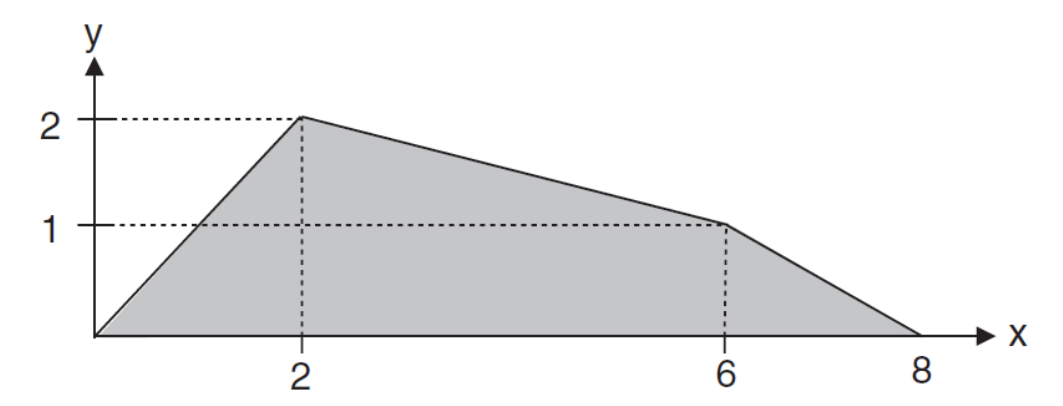
\includegraphics[width=0.75\textwidth]{figure_from_instruction.png}
\end{figure}

\subsection*{Rozwiązanie}

Symulacja została zaprogramowana w języku Python, jako funkcja\\ 'monte\_carlo\_square\_aproximation' w pliku 'simulation.py'.
Kod tej symulacji przedstawiono poniżej.
\begin{verbatim}
  def monte_carlo_square_aproximation(runs, a, b):
    xs = np.random.uniform(0, a, runs)
    ys = np.random.uniform(0, b, runs)

    inFigure = ((xs <= 2) & (ys <= xs)) | (((xs > 2) & (xs <= 6)) 
      & (ys <= -(xs/4)+2.5))  | ((xs > 6) & (ys <= -(xs/2)+4))

    mcArea = (sum(inFigure) / runs) * (a*b)

    return mcArea, xs, ys, inFigure
\end{verbatim}

Funkcja ta przyjmuje trzy parametry:
\begin{itemize}
  \item runs - ilość punktów generowanych w ramach symulacji
  \item a - długość obszaru symulacji (jako wartość osi x)
  \item b - wysokość obszaru symulacji (jako wartość osi y)
\end{itemize}

Generuje ona za pomocą metody z pakietu "numpy" losowe punkty w zakresie od 0 do "a" dla osi "x" oraz od 0 do "b" dla osi "y". Ilość punktów wyznacza wartość "runs".

Nastepnie funkcja tworzy listę wartości prawda/fałsz określającą przynależność poszczególnych punktów do figury. Granice figury od dołu wyznacza oś "x", od góry natomiast jest ona ograniczona trzema funkcjami linowymi:

\begin{itemize}
  \item dla $x <= 2$ funkcją $y = x$
  \item dla $2 < x <= 6$ funkcją $y = -(x/4) + 2.5 $
  \item dla $x > 6$ funkcją $y = -(x/2) + 4$
\end{itemize}

W ostatnim etapie funkcja ta używając symulacji Monte Carlo wyznacza przybliżoną powierzchnię figury.

\subsection*{Wyniki}

Na początek wyliczono prawidłową wartość stosując zasady matematyczne i dzieląc figurę na 3 trójkąty i jeden prostokąt.
\begin{gather*}
  P_1 = 1 * 4\\
  P_1 = 4
\end{gather*}
\begin{gather*}
  P_2 = \frac{2 * 2}{2} \\
  P_2 = 2
\end{gather*}

\begin{gather*}
  P_3 = \frac{1 * 4}{2} \\
  P_3 = 2
\end{gather*}

\begin{gather*}
  P_4 = \frac{1 * 2}{2} \\
  P_4 = 1
\end{gather*}

Ostatecznie po zsumowaniu otrzymano wynik $P = P_1 + P_2 + P_3 + P_4 = 4 + 2 + 2 + 1 = 9$, który stanowić będzie punkt odniesienia dla oceny aproksymacji.

Dla pojedynczego przebiegu symulacji uzyskano wynik $mc\_area = 8.9438$ co przedstawiono na poniższym rysunku. Zatem błąd aproksymacji dla 100000 punktów wynosi $\epsilon = 9 - 8.9438 = 0.0562$

\begin{figure}[H]
  \centering
  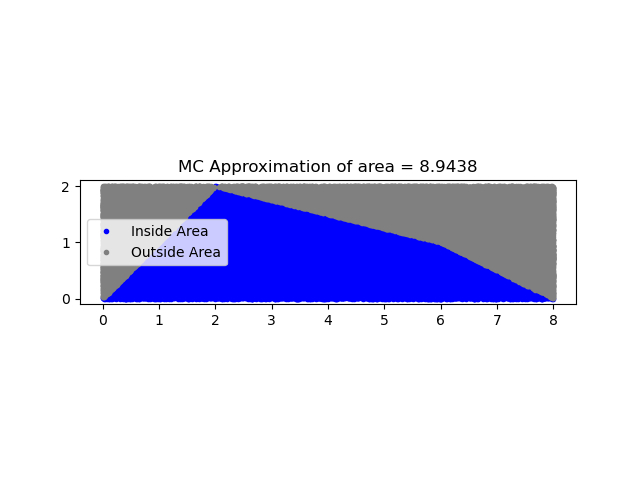
\includegraphics[width=0.75\textwidth]{area_aproximation_single_run.png}
\end{figure}

Dla uzyskania dokładniejszego i pewniejszego resultatu, przeprowadzono 100 symulacji i obliczono wartosć odchylenia standardowego. Odchylenie jak zaprezentowano poniżej wyniosło $\sigma = 0.024064594460742418$.

\begin{verbatim}
  Simulation count: 100
  Standard deviation: 0.024064594460742418
\end{verbatim}

\subsection*{Wnioski}

Jak można zauważyć aproksymacja pola powierzchni figur przy pomocy symulacji Monte Carlo daje wyniki bardzo zbliżone do rzeczywistego pola powierzchni. Wyniki te jednak nie są wartością dokładną.

Dla większości przypadków końcowy błąd mieści się w granicach statystycznych i pozwala z powodzeniem stosować symulacje Monte Carlo do obliczania pola powierzchni figur.

\end{document}